\subsection{Hardware}
The smart wheelchair should have the ability to sense, process, and manoeuvre within the surrounding environment.
To do this requires some necessary hardware, including a sensor system, compute element, and motor controller.
Due to the 2021-2022 chip shortage, hardware selection was identified as a process that should occur relatively quickly.

The literature review provides a comparison between different sensor types and models. For outdoor navigation assistance,
a forward-facing RGB-D camera was selected as the best option for this project - specifically, the Zed 2 Mini.
This was chosen due to the high resolution provided by RGB-D cameras, and the long-distance range of the Zed cameras due to 
their passive operation (does not use an IR emitter).

% Should this be in the methodology?
The front of the joystick control unit was selected as the best mounting point for the
stereo camera, due to several reasons:
\begin{enumerate}[topsep=0pt,itemsep=-1ex,partopsep=1ex,parsep=1ex]
    \item Clear view of the environment in front of the wheelchair.
    \item Not obstructed by the user in any wheelchair configuration.
    \item When needed, the user can move the joystick control unit out of the way,
            which also moves the camera out of the way.
\end{enumerate}
However, there are some challenges faced when using this mounting point, which must be addressed.
\begin{enumerate}[topsep=0pt,itemsep=-1ex,partopsep=1ex,parsep=1ex]
    \item Shaky video footage due to low rigidity in joystick mount.
    \item Close to the front of the wheelchair, which reduces the visibility of the sides of the wheelchair.
    \item Maximum camera width of \SI{150}{\milli\metre} before doorway manoeuvrability is affected.
\end{enumerate}
Due to the size constraints, the Mini form factor was chosen.

An additional sensor with a wider field of view will be needed for doorway navigation
and wheelchair docking, due to the limitations of this mounting point. The sensor selected for this purpose
was a 2D Lidar unit attached to the base of the wheelchair. However, this sensor will not be used for
our specific application (pathway assistance).

For the compute element, an Nvidia Jetson Xavier NX will be used, due to compatibility with the Zed API
and a wide range of ML frameworks, as well as low power use.
The motor controller is being designed by a different thesis student; \cref{fig:block_diagram} shows
how it integrates with other hardware on the wheelchair.

\subsection{Dataset Collection}
To train and evaluate machine learning models, a stereo camera dataset will be collected by driving the wheelchair
around Curtin University. This dataset will provide valuable RGB and depth information, as well as movement data
from an inbuilt IMU. A preliminary video dataset will also be collected before the stereo camera is purchased,
to enable the initial evaluation of scene recognition algorithms.

\subsection{Software}
%Our software system requires several components. Interaction with the Zed 2 Mini will be done
%via the proprietary Stereolabs API, which will provide RGB-D imaging to the computer.
The software system will involve a series of scene recognition algorithms to build and update an occupancy map of the surrounding area.
Interaction with the Zed 2 Mini will be done using the proprietary Stereolabs API, and
PyTorch \cite{paszkePyTorchImperativeStyle2019} will be used for training and evaluation of machine learning models.
PyTorch provides good compatibility with existing machine learning models such as YOLOv5 \cite{ultralyticsYOLOv5} and DeepLabv3 \cite{chenRethinkingAtrousConvolution2017}.

Assistive control algorithms will then be used to choose the direction and speed of the wheelchair, based on the occupancy map and the user's desired direction.
Several machine learning and assistive control algorithms will be evaluated based on their
speed and accuracy to choose which are suitable for the final software implementation.

An embedded microcontroller system and motor controller are being designed by other thesis students,
which will allow the software system to communicate with the underlying wheelchair hardware in a standard way.
The embedded microcontroller will validate the chosen direction and speed of the wheelchair, to ensure
that in the case of a software failure the user is still able to use the wheelchair. \Cref{fig:block_diagram}
shows a block diagram of the final semi-autonomous wheelchair design.

As the timeline of the embedded microcontroller system is uncertain, a basic simulation environment for the software system will be created.
This allows the performance of the autonomous system to be validated without reliance on other thesis projects.
% System diagram
\begin{figure}[H]
    \centering
    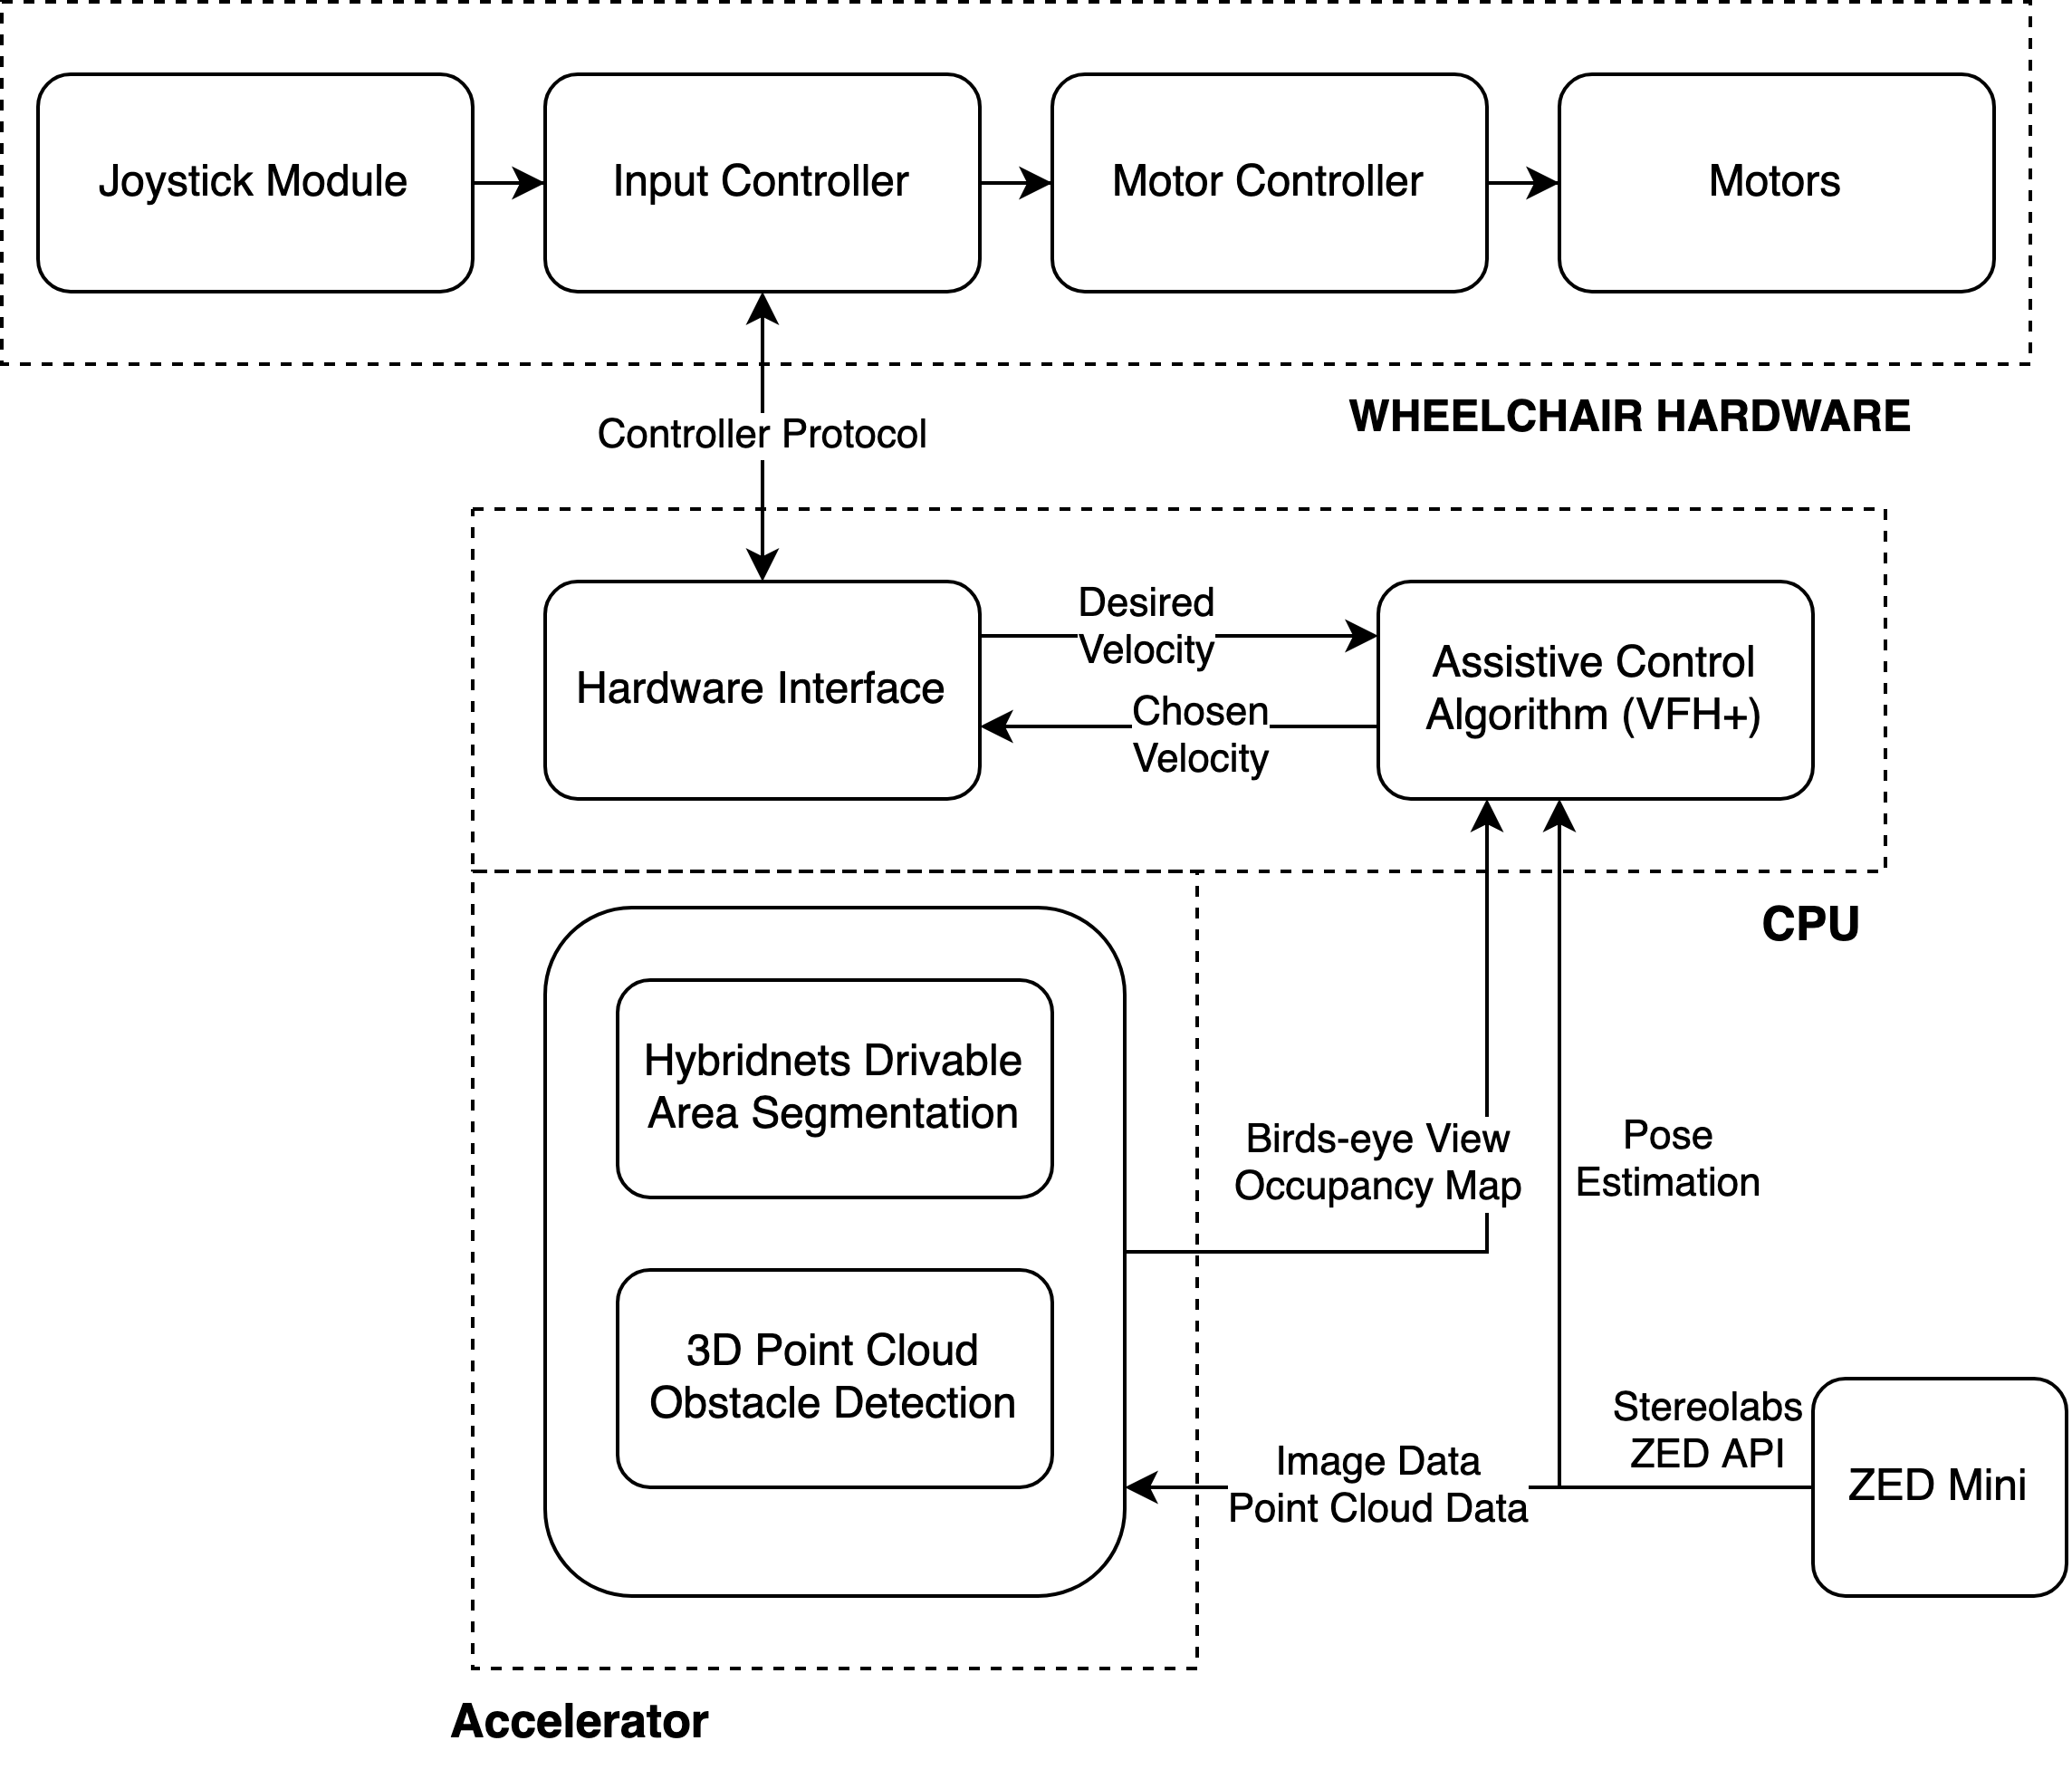
\includegraphics[width=\linewidth]{images/block_diagram.png}
    \caption{Block diagram of system}
    \label{fig:block_diagram}
\end{figure}
\pagebreak

\subsection{Time Planning}
Time should be allocated to thesis writing and review as well as technical progress.
A Gantt chart displaying the expected progress over the course of the two semesters
is shown in \cref{fig:gantt_chart}. Note that a significant portion of time at the beginning was allocated
to initial research and project scope. Due to the large number of students working on this team,
a clear project scope was important so that students did not unnecessarily duplicate work.

\begin{figure}[H]
    \centering
    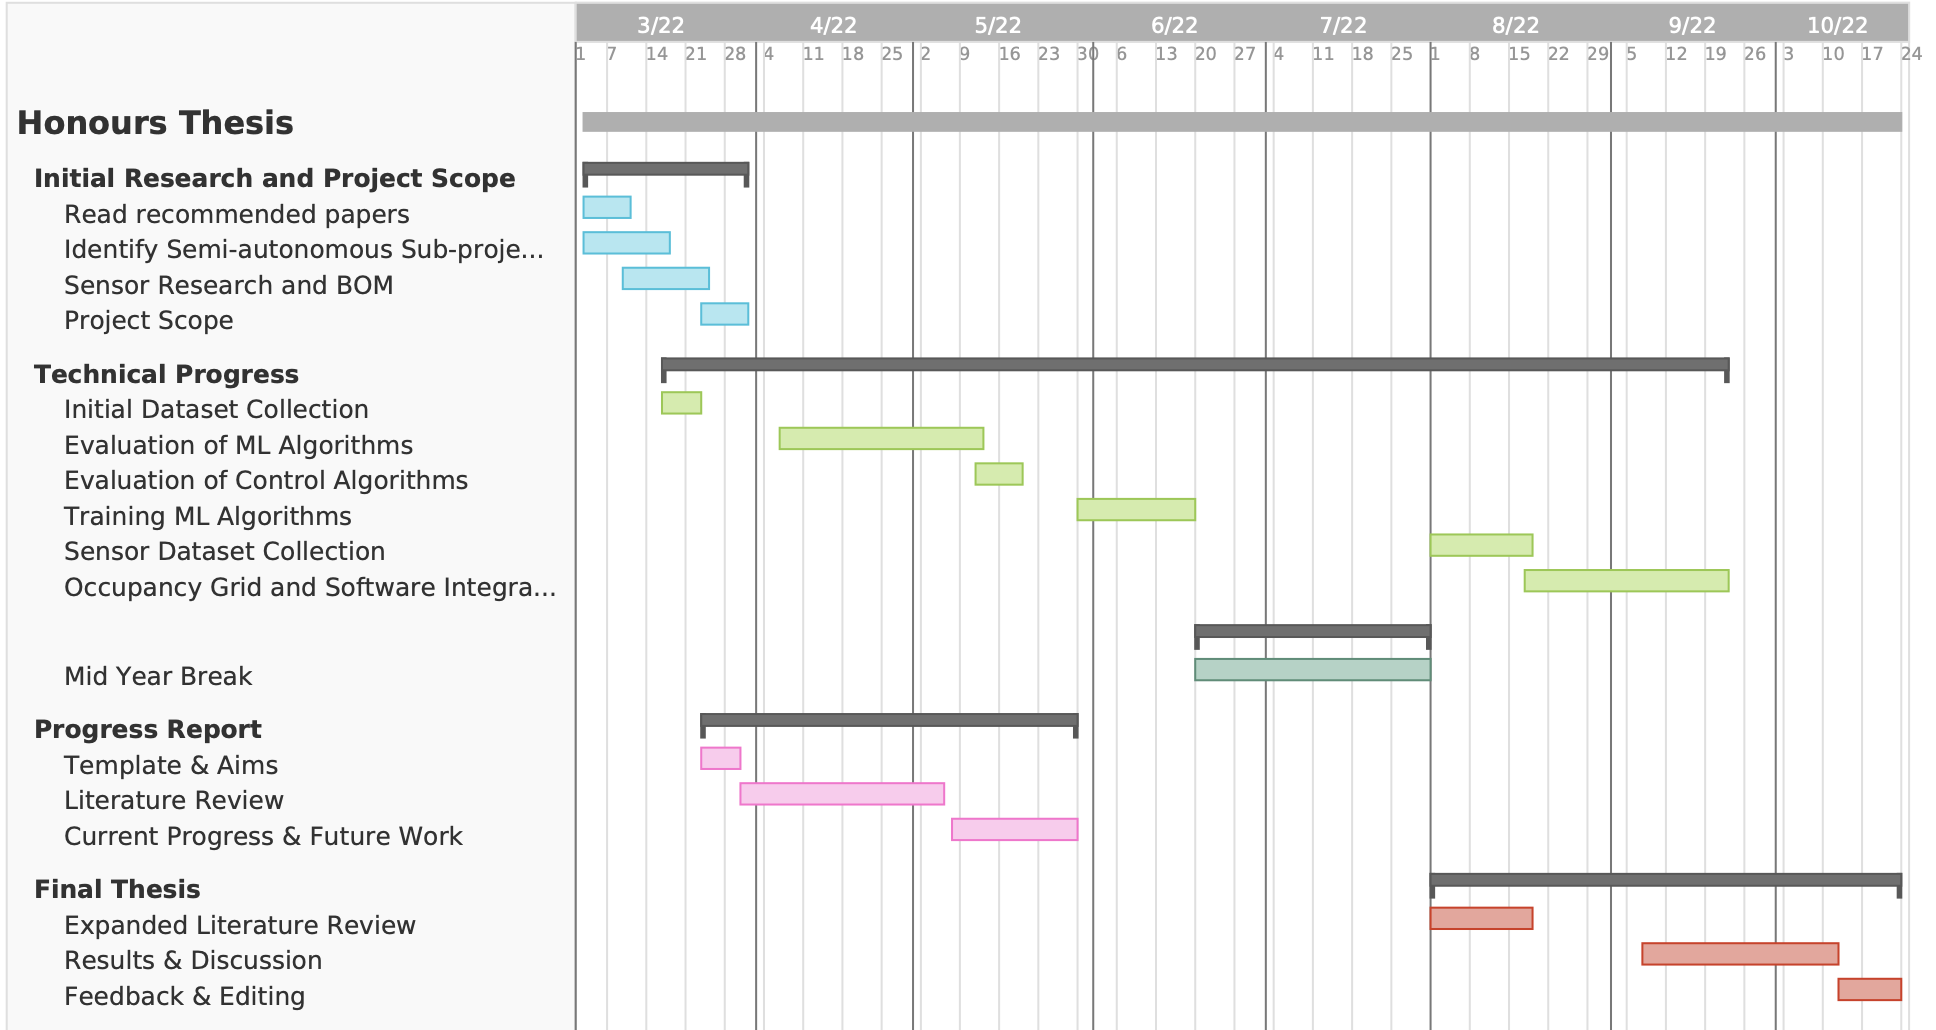
\includegraphics[width=\linewidth]{images/gantt_chart.png}
    \caption{Gantt chart of thesis progress}
    \label{fig:gantt_chart}
\end{figure}
